\section{Trees}
\subsection{Introduction to trees}
\begin{center}
  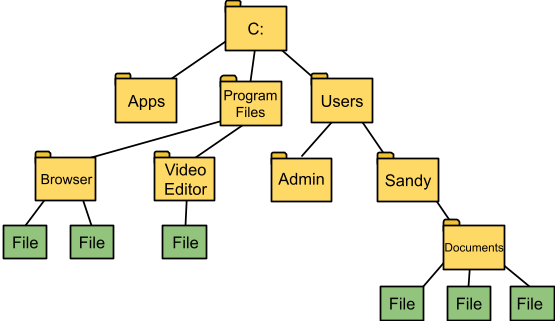
\includegraphics[width=0.6\linewidth]{resources/diagram of a file system.png}
\end{center}
The file system can be seen as a graph in which each folder or file is a vertex. There is an edge between two folders if one folder is a subfolder of the other. There is an edge between a file and a folder if the file resides in that folder. In most computer operating systems, a file or folder can only reside in one location, which means that the underlying graph corresponds to a tree.

\subsubsection*{Definition of a Tree}
A \bld{tree} is an undirected graph that is connected and has no cycles.

\subsubsection*{Free Trees and Rooted Trees}
\begin{center}
  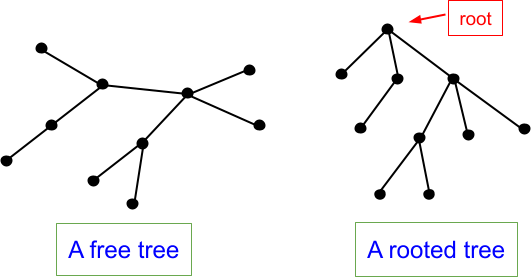
\includegraphics[width=0.5\linewidth]{resources/free and rooted trees.png}
\end{center}
The tree on the left is called a \bld{free tree} because there is no particular organization of the vertices and edges. The tree on the right is called a \bld{rooted tree}. The vertex at the top of the drawing is designated as the \bld{root} of the tree. The remaining vertices are organized according to their distance from the root. The distance between two vertices in an undirected graph is the number of edges in the shortest path between the two vertices. The \bld{level} of a vertex is its distance from the root. The \bld{height} of a tree is the highest level of any vertex. The tree on the right has height 3.

\subsubsection*{Theorem: Unique Paths in Trees}
Let $T$ be a tree and let $u \tand v$ be two vertices in $T$. There is \itl{exactly one path} between $u \tand v$.

\subsubsection*{Terminology related to Rooted Trees}
\begin{itemize}
  \item Every vertex in a rooted tree $T$ has a unique \bld{parent}, except for the root which does not have a parent. The parent of vertex $v$ is the first vertex encountered along the path from $v$ to the root.
  \item Every vertex along the path from $v$ to the root, except for the vertex $v$ itself, is an \bld{ancestor} of vertex $v$.
  \item If $v$ is the parent of vertex $u$, then $u$ is a \bld{child} of vertex $v$.
  \item If $u$ is an ancestor of $v$, then $v$ is a \bld{descendant} of $u$.
  \item A \bld{leaf} is a vertex which has no children.
  \item Two vertices are \bld{siblings} if they have the same parent.
  \item A \bld{subtree} rooted as vertex $v$ is the tree consisting of $v$ and all of $v$'s descendants.
\end{itemize}

\subsubsection*{Forests}
A \bld{forest} is a graph that has no cycles but is not necessarily connected. The picture below shows a forest with 3 connected components.
\begin{center}
  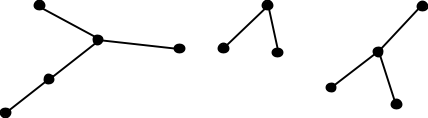
\includegraphics[width=0.6\linewidth]{resources/forest example.png}
\end{center}

\subsection{Tree application examples}

\subsubsection*{Game Trees}
\begin{center}
  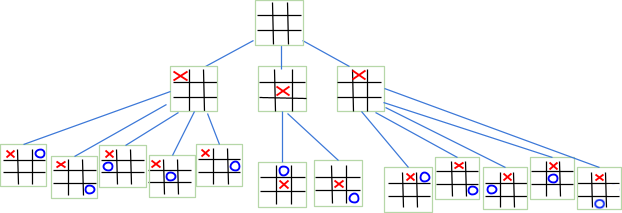
\includegraphics[width=0.7\linewidth]{resources/tictactoe game tree.png}
\end{center}
The root of the tree is the initial configuration of the game. In the case of tic-tac-toe, the initial configuration is an empty grid. The odd levels of the game tree represent choices of play for the X player and the even levels represent choices of play for the O player. The children of a configuration c are all the configurations that can be reached from c by a single move of the correct player. A configuration is a leaf vertex in the tree if the game is over.

Theoretically, a game tree can be systematically analyzed to determine optimal playing strategies for each player. However, in practice for most games, the corresponding game tree is much too large to build and analyze in its entirety. Programs like Deep Blue build partial game trees starting from the current configuration in the game and estimate the best next move based on the results of the partial tree.

Tic-tac-toe and chess are examples of deterministic games whose outcome is completely determined by the choices made by each player. A game that involves rolling a pair of dice or shuffling a deck of cards introduces randomization into the game. Probability theory as well as game trees are required to analyze games with an element of chance.

\subsubsection*{Prefix Codes}
Space-efficient encodings can be achieved by \bld{variable length codes}, in which the number of bits for each character can vary. Characters such as "a" and "e" that occur frequently are represented with fewer bits, while characters such as "z" or "q" are represented using more bits.

Trees are a convenient way to represent variable length codes for translating between text and binary.
\begin{center}
  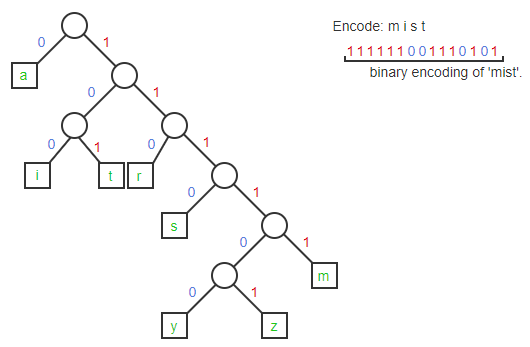
\includegraphics[width=0.6\linewidth]{resources/variable length encoding example.png}
\end{center}
The code illustrated in the animation is an example of a prefix code. A string $s$ is a \bld{prefix} of another string $t$ if all the characters in string $s$ appear at the beginning of string $t$.
\begin{center}
  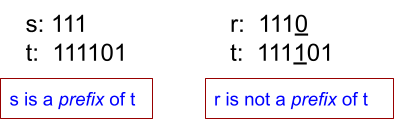
\includegraphics[width=0.4\linewidth]{resources/string prefix example.png}
\end{center}
A \bld{prefix code} has the property that the code for one character \itl{can not} be a prefix of the code for another character. The fact that the codes are organized as a tree in which characters are only stored at the leaves ensures the prefix property.

\subsection{Properties of trees}

\subsubsection*{Theorem: Unique Paths in Trees}
There is a unique path between every pair of vertices in a tree.

\subsubsection*{Theorem: Number of Leaves in a Tree}
Any free tree with at least two vertices has at least two leaves.

\subsubsection*{Theorem: Number of Edges in a Tree}
Let $T$ be a tree with $v$ vertices and $e$ edges. Then
\[
  e = v-1.
\]

\subsection{Tree traversals}
A common procedure performed on a tree, called a \bld{tree traversal}, is to process the information stored in the vertices by systematically visiting each vertex. In a \bld{pre-order traversal}, a vertex is visited before its descendants. In a \bld{post-order traversal}, a vertex is visited after its descendants.

\subsubsection*{Pseudocode and Example for Pre-order Traversal}
\begin{lstlisting}
Pre-order(v)

process(v) // process happens first
For every child w of v:
  Pre-order(w)
End-for
\end{lstlisting}
\begin{center}
  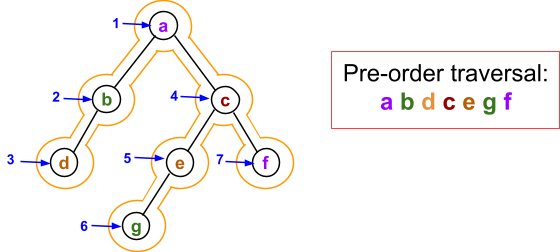
\includegraphics[width=0.4\linewidth]{resources/preorder traversal.png}
\end{center}

\subsubsection*{Pseudocode and Example for Post-order Traversal}
\begin{lstlisting}
Post-order(v)

For every child w of v:
  Post-order(w)
End-for
process(v) // process happens last
\end{lstlisting}
\begin{center}
  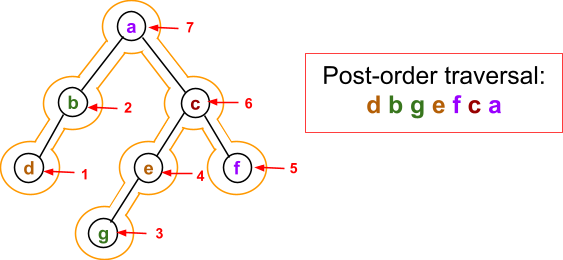
\includegraphics[width=0.4\linewidth]{resources/post order traversal.png}
\end{center}

\subsection{Spanning trees and graph traversals}
Suppose an application needs to broadcast information to every computer (vertex) in a network. The information will be disseminated along the communication links so that every vertex in the network receives the information. Moreover, the goal is to minimize overall congestion, so it would be wasteful to send information along alternate paths to the same location. The information should be broadcast over a spanning tree of the network. Here is the formal definition of a spanning tree:

\subsubsection*{Definition of a Spanning Tree of a Connected Graph}
A \bld{spanning tree} of a connected graph $G$ is a subgraph of $G$ which contains all the vertices in $G$ and is a tree.

\subsubsection*{}
The picture below shows several possible spanning trees of the same graph. The edges of the spanning tree are shown in red. The vertex set of the spanning tree is always the entire set of vertices in the graph.
\begin{center}
  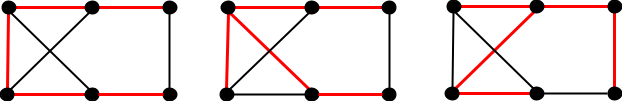
\includegraphics[width=0.6\linewidth]{resources/spanning trees example.png}
\end{center}

\subsubsection*{Graph Traversals}
There are two common methods for finding spanning trees in a graph: Breadth-First Search and Depth-First Search. Both methods start at a single vertex and incrementally build a connected tree by adding edges and vertices. The resulting tree is rooted at the start vertex. Graph traversal is a process that systematically explores all the vertices of a graph.

\subsubsection*{Depth-First Search}
As the name suggests, Depth-First Search (DFS) favors going deep into the graph and tends to produce trees with longer paths from the start vertex.
\begin{lstlisting}
Depth-first-search

Input: An undirected, connected graph G. A start vertex v[1]
Output: T, a depth-first search tree.

Add v[1] to T.
visit(v[1])

visit(v)

For every neighbor w of v:
  If w is not already in T
    Add w and {w, v} to T.
    visit(w);
  End-if
End-for
\end{lstlisting}
Note that there is some ambiguity with regard to the order in which the neighbors of a vertex are considered.

\subsubsection*{Breath-first Search}
Breadth-First Search (BFS) explores the graph by distance from the initial vertex, starting with its neighbors and expanding the tree to neighbors of neighbors, etc. Breadth-first-search visits vertices in the graph according to their proximity to the start vertex. The algorithm maintains a list of vertices to be visited soon. Vertices are added to the back of the list and the next vertex to visit is taken from the front of the list.
\begin{lstlisting}
Breadth-first-search

Input: An undirected, connected graph G. A start vertex v[1]
Output: T, a breadth-first search tree.

Add v[1] to T.
Add v[1] to the back of the list.

While the list is not empty:
  Remove vertex v from the front of the list.
  For each neighbor w of v that is not already in T:
    Add w and {w, v} to T.
    Insert w at the back of the list.
  End-for
End-while
\end{lstlisting}

\subsection{Minimum spanning trees}
When edges have varying costs, a natural goal is to minimize the total cost of the spanning tree.

\subsubsection*{Definition of a Weighted Graph}
A \bld{weighted graph} is a graph $G = (V,E)$, along with a function $w: E \rightarrow \bb{R}$. The function $w$ assigns a real number to each edge.
\begin{center}
  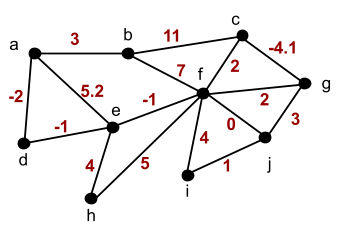
\includegraphics[width=0.6\linewidth]{resources/example weighted graph.png}
\end{center}
When the goal is to span the vertices of the graph while minimizing the total weight of the edges used, a \bld{minimum spanning tree} can be used.

\subsubsection*{Definition of a Minimum Spanning Tree}
A \bld{minimum spanning tree} (MST) of a weighted graph is a spanning tree $T$ of $G$ whose weight is no larger than any other spanning tree of $G$.

\subsubsection*{Prim's Algorithm for Minimum Spanning Trees}
This is a classic algorithm for finding minimum spanning trees, developed by mathematician Robert Prim in 1957.
\begin{lstlisting}
Input: An undirected, connected, weighted graph G.
Output: T, a minimum spanning tree for G.

T := {}.
Pick any vertex in G and add it to T.

For j = 1 to n-1
  Let C be the set of edges with one endpoint inside T 
      and one endpoint outside T.
  Let e be a minimum weight edge in C.
  Add e to T.
  Add the endpoint of e not already in T to T.
End-for
\end{lstlisting}

\subsubsection*{Theorem: Result of Prim's Algorithm}
Prim's algorithm finds a minimum spanning tree of the input weighted graph.